\section{Pressure management}
\label{sec:pressure_management}
As mentioned previously, pressure management is a method that ensures the customers with the minimum water pressure, while reducing the excessive pressure on the pipes from the water supply network. Which will reduce the probability of leakage or new pipe bursts.
\\
\\
In pressure management there exist several systems and technologies. The system is usually set up by dividing the distribution network into smaller areas, which are called pressure management areas (PMA). PMAs can either cover a city block, an industrial area or any other area that needs to be supplied from the distribution network. A PMA is connected to the distribution network via a pressure reduction valve (PRV), which reduces the pressure inside the PMA. The PRV has the purpose of maintaining a minimum pressure at the critical point (CP) inside the PMA. The CP is defined as the end user in the PMA and requires a certain minimum pressure, so the end user at the CP, can use the water \cite{guidelines_waterloss}.   
\\
The PRVs exist in many variants from more advanced PRVs, which can be time dependent to accommodate for daily variation in water use or remote controlled by a operator from a monitor to a more basic one that works like a pressure drop from the distribution network to the PMA.
\\
\\
In the next part, two examples for pressure reduction in a PMA will be presented, one of which is using a basic PRV and another one using pumps. 
\\
Figure \ref{fig:prv} illustrates a distribution network leading into a PMA which has a PRV to regulate the water pressure into the CP.  
\begin{figure}[H]
\centering
\includegraphics[width=0.9\textwidth]{report/introduction/pictures/PRV.png}
\caption{ Show that the pressure from the distribution network to the PMA is reduced by a PRV \cite{guidelines_waterloss}.}
\label{fig:prv}
%Kilde for Figur:  http://forsvaret.dk/MST/NATIONALT/SOEREDNING/UNDERAFKOELING/Pages/default.asps
\end{figure}

As shown on figure \ref{fig:prv}, the pressure drops after the PRV and therefore the pressure into the PMA at the CP gets lowered, which means that the pressure is lower than it would have been if the water came directly from the reservoir. If the water came directly from the reservoir, the pressure would have been much higher at the CP and it could have caused increased water loss and damage to the distribution network. A downside of PRV is that it reduces the pressure which means that it consumes the energy that has been used in the water reservoir to increase the pressure. 
\\
\\
Figure \ref{fig:pump} illustrates the same network as figure \ref{fig:prv} but with a pump instead of a PRV.

\begin{figure}[H]
\centering
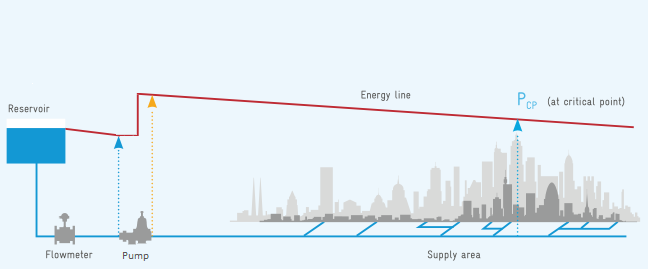
\includegraphics[width=0.9\textwidth]{report/introduction/pictures/pump.png}
\caption{ The pressure from the distribution network to the PMA is increased by a pump. The figure is from \cite{guidelines_waterloss} but with changes, that have been made to illustrate the point of pressure management with a pump. The original figure \cite{guidelines_waterloss} has been modified to fit the needs of the report.}
\label{fig:pump}
%Kilde for Figur:  http://forsvaret.dk/MST/NATIONALT/SOEREDNING/UNDERAFKOELING/Pages/default.asps
\end{figure}

The pump on figure \ref{fig:pump} is used to boost the pressure into the PMA which enables the water reservoir able to use less energy on creating a certain amount of water pressure. A problem arises when using pumps instead of PRV: when several pumps are connected to the same network, instability can occur when feedback control is used for the pump.  

%The figure \ref{fig:pump} shows that the pressure from the reservoir is lower than it was on figure \ref{fig:prv} that is because of the pump will increase the pressure so it meets the required pressure at CP. This method has the advantage that it does not lower the pressure like on figure \ref{fig:prv} and therefore it does not waste energy on lowering the pressure.  



